%%%%%%%%%%%%%%%%%%%%%%%%%%%%%%%%%%%%%%%%%
% Medium Length Professional CV
% LaTeX Template
% Version 2.0 (8/5/13)
%
% This template has been downloaded from:
% http://www.LaTeXTemplates.com
%
% Original author:
% Trey Hunner (http://www.treyhunner.com/)
%
% Important note:
% This template requires the resume.cls file to be in the same directory as the
% .tex file. The resume.cls file provides the resume style used for structuring the
% document.
%
%%%%%%%%%%%%%%%%%%%%%%%%%%%%%%%%%%%%%%%%%

%----------------------------------------------------------------------------------------
%	PACKAGES AND OTHER DOCUMENT CONFIGURATIONS
%----------------------------------------------------------------------------------------

\documentclass{resume} % Use the custom resume.cls style
\usepackage[dvipsnames]{xcolor}
\usepackage{gensymb}
\usepackage{graphicx}

\usepackage[left=0.75in,top=0.55in,right=0.75in,bottom=0.1in]{geometry} % Document margins
\newcommand{\tab}[1]{\hspace{.2667\textwidth}\rlap{#1}}
\newcommand{\itab}[1]{\hspace{0em}\rlap{#1}}
\name{Jeremy K. Thaller} % Your name
\address{ Acton, MA 01720 \\ jthaller.github.io/portfolio } % Your address
%\address{123 Pleasant Lane \\ City, State 12345} % Your secondary addess (optional)
%\address{github: jthaller \\ }
\address{+1 978-496-7990 \\ jkt2@alumni.williams.edu} % Your phone number and email
%\definecolor{darkpurple}{RGB}{108,48,130}

\renewenvironment{rSection}[1]{
	\sectionskip
	\textcolor{RoyalPurple}{\MakeUppercase{#1}}
	\sectionlineskip
	\hrule
	\begin{list}{}{
			\setlength{\leftmargin}{1.5em}
		}
		\item[]
	}{
	\end{list}
}

\begin{document}


%\begin{flushright}
%	\vspace{-3cm}
%	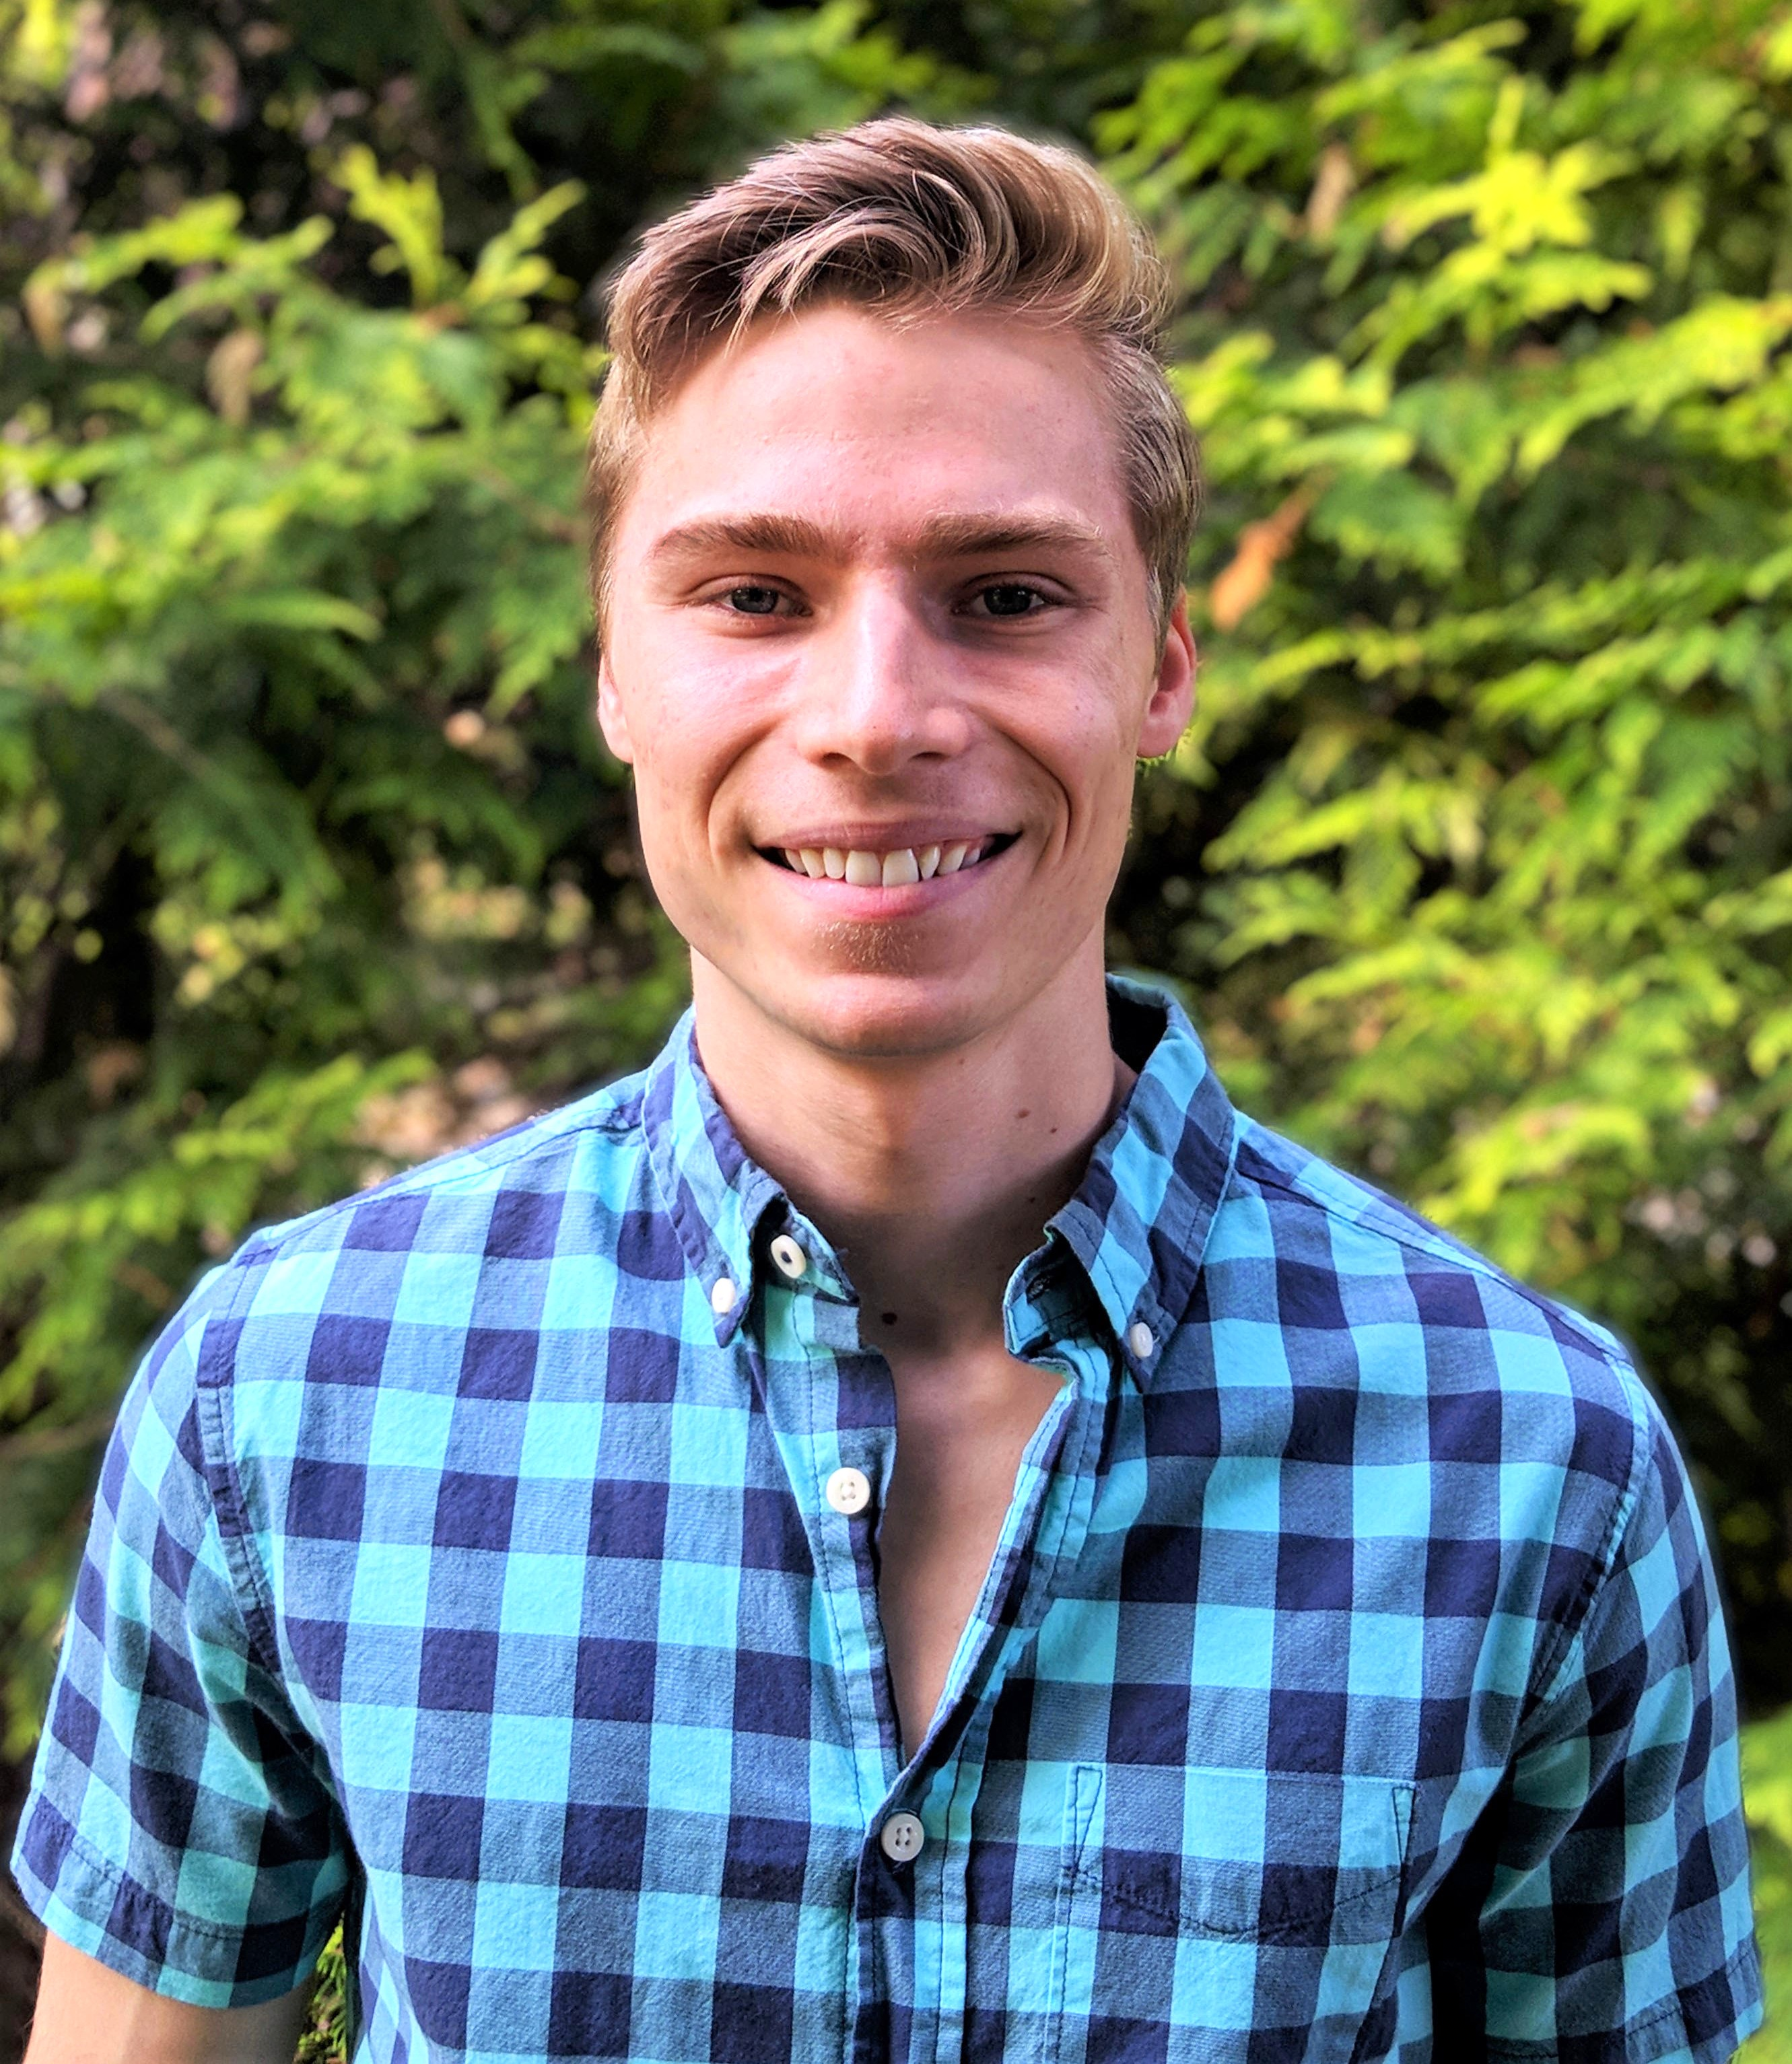
\includegraphics[width=3cm]{Jeremy_headshot_cropped.jpg}
%	\vspace{-1cm}
%\end{flushright}


	%----------------------------------------------------------------------------------------
	%	EDUCATION SECTION
	%----------------------------------------------------------------------------------------
\vspace{-2em}
	\begin{rSection}{Education} 
		
		\begin{rSubsection}{Erasmus Mundus: Dual Degree Master's Program}{\em In Progress}{}{}
				\vspace{-.4em}
				\item[] Expected Graduation: September 2021
				\vspace{-.4em}
		\end{rSubsection}
				\begin{rSubsection}{\hspace{.04\textwidth} Adam Mickiewicz University, Pozna\'n}{\em 2020 -- 2021}{}{}
					\vspace{-.4em}
					\item[] \hspace{.04\textwidth} MSci. in Physics of Advanced Materials for Energy Processing
				\end{rSubsection}
				\vspace{-.3em}
				\begin{rSubsection}{\hspace{.04\textwidth} Ludwig Maximilians Universit{\"a}t  M{\"u}nchen (LMU) \&}{}{}{}
					\item[] \vspace{-2.75em}
				\end{rSubsection}
%				\vspace{-.5em}
				\begin{rSubsection}{\hspace{.04\textwidth} Technische Universit{\"a}t M{\"u}nchen (TUM)}{\em 2019 -- 2020}{}{}
					\vspace{-.4em}
					\item[] \hspace{.04\textwidth} Joint MSci. in Geomaterials and Geochemistry
				\end{rSubsection}
		
%		\begin{rSubsection}{Adam Mickiewicz University, Poznan}{\em In Progress}{}{}
%			\vspace{-.5em}
%			\item MSci. in Physics of Advanced Materials for Energy Processing
%		\end{rSubsection}
%		
%		\begin{rSubsection}{Ludwig Maximilians Universit{\"a}t  M{\"u}nchen (LMU) \&\\Technische Universit{\"a}t M{\"u}nchen (TUM)}{\em 2019 -- 2020}{}{}
%			\vspace{-.5em}
%			\item Joint MSci. in Geomaterials and Geochemistry
%		\end{rSubsection}
\vspace{-.4em}
		\begin{rSubsection}{Williams College}{\em 2015 -- 2019}{}{}
			\vspace{-.4em}
			\item[] B.A. in Physics with Honors
			\item[] Pre-engineering Studies
			\item[] Sigma Xi Honors Society Inductee
		\end{rSubsection}

		\begin{rSubsection}{Acton-Boxborough Regional High School}{\em 2011 -- 2015}{}{}
			\vspace{-.4em}
			\item[] National AP Scholar
			\item[] National Honors Society
		\end{rSubsection}

\vspace{-1.2em}
	\end{rSection}
	%----------------------------------------------------------------------------------------
	%	TECHNICAL STRENGTHS SECTION
	%----------------------------------------------------------------------------------------
	\newcommand{\CC}{C\nolinebreak\hspace{-.05em}\raisebox{.4ex}{\tiny\bf +}\nolinebreak\hspace{-.10em}\raisebox{.4ex}{\tiny\bf +}}
	\def\CC{{C\nolinebreak[4]\hspace{-.05em}\raisebox{.4ex}{\tiny\bf ++}}}

	\begin{rSection}{Technical Strengths}
	
	\begin{tabular}{ @{} >{\bfseries}l @{\hspace{6ex}} l }
		Programming Languages &  Python, MATLAB, JAVA, SQL, Arduino (C/\CC) \\
		Python Packages & Pandas, NumPy, Scikit-Learn, PyTorch, Tensorboard, KERAS, \\
		& TensorFlow, Seaborn, Regex, Optuna  \\
		Data Software & Mathematica, Quantum Espresso, Excel, LabView, LoggerPro \\
		Visualization Software & LaTeX, Solid Works, VESTA, Full Prof, Adobe Illustrator, Photoshop \\
		Machining Experience & Bridgeport Milling, CNC Milling, 3D Printing, Laser Cutting, \\
		& Arc Melting, Fluorescent Confocal Microscopy, SEM, TEM, XRD
	\end{tabular}
	
	\end{rSection}
\vspace{-1.2em}
%------------------------------------------------------------------------------------
%       Projects
%------------------------------------------------------------------------------------
\begin{rSection}{Data Science Projects} \itemsep -2pt
	\begin{tabular}{ @{} >{}l @{\hspace{6ex}} l }
		Facebook Messenger Statistics and Word-Cloud Plots & Spam Email Classifier\\
		Chatbot based on personal Messanger Data & Quora Spam Question Identifier \\ 
		Semiconductor Optimization Predictor & Covid-19 Case Forecasting \\
		CIFAR-10 Classifier & Image Segmentator
	\end{tabular}
\end{rSection}

	%----------------------------------------------------------------------------------------
	%	RESEARCH EXPERIENCE SECTION
	%----------------------------------------------------------------------------------------

\vspace{-1em}
	\begin{rSection}{Research Experience}
		\begin{rSubsection}{Amorphous Solids, Metallic Glasses, \& Metallurgy}{Summer 2019}{Postbac Researcher}{}
			\vspace{-.5em}
			\item[] {\em Advised by Jan Schroers, Professor of Mechanical Eng. \& Materials Science}\hfill {\em Yale University}
			\item Arc-melted complex shape memory and eutectic alloys.
			\item Nano-molded crystalline metals to determine the underlying mechanism.
			\item Measured atomic surface properties with SEM and determined crystal orientation with TEM
		\end{rSubsection}


		\begin{rSubsection}{Soft Condensed Matter Physics}{May 2018 -- June 2019}{Undergraduate Honors Thesis}{}
			\vspace{-.5em}
				\item[] {\em Advised by Katharine E. Jensen, Professor of Physics}\hfill {\em Williams College}
				\item Designed and built stretching apparatus to induce equibiaxial stretch in soft materials
				\item Collected data via Fluorescent Confocal Microscopy 
				\item Analyzed data through modified MATLAB scripts to measure the strain dependency of solid surface stress in soft materials via adhesion

		\end{rSubsection}

		\pagebreak

		\begin{rSubsection}{Atomic, Molecular, and Optical Physics}{Summer 2017}{Undergraduate Research Assistant}{}
			\vspace{-.5em}
			\item[] {\em Advised by Protik K. Majumder, Professor of Physics}\hfill {\em Williams College}
			\item Took data towards an ultra-precise  measurement of the Electric Quadrupole (E2) amplitude within the $6S^26P^2$ $^3P_0$ $\rightarrow$ $^3P_2$ transition in Pb
			\item Programed a PID controller in LabView to thermally regulate an oven to within $\pm .4\degree$ C at temperatures near $ 950\degree $ C
			\item Designed a deposition-rate detector for an indium cell chamber based on the mass dependent frequency of Quartz Crystals
		\end{rSubsection}

\end{rSection}

%------------------------------------------------------------------------------------
%       Data Science Skills
%------------------------------------------------------------------------------------
%\begin{rSection}{Data Science Skills} \itemsep -2pt
%	\begin{tabular}{ @{} >{}l @{\hspace{6ex}} l }
%		Python & MATLAB \\
%		Data Visualization & Data Cleaning and Feature Engineering \\
%		Command Line (BASH) & Probability and Statistics \\ 
%		SSH + EMACS & Git and Version Control \\
%	\end{tabular}
%\end{rSection}


%------------------------------------------------------------------------------------
%       WORK EXPERIENCE
%------------------------------------------------------------------------------------
\begin{rSection}{Other Work Experience} \itemsep -2pt
	\begin{rSubsection}{Office of Information Technologies}{June 2017 -- Aug. 2017}{}{Williams College}{}
		\item {Student Technology Assistant} \hfill {\em 40 hr/week}
	\end{rSubsection}
	%-----------------------------
	\begin{rSubsection}{Williams College Wind Ensemble}{Sept. 2016 -- June 2017}{}{Williams College}{}
		\item {Teaching Assistant, Bassoonist} \hfill {\em 40 hr/week}
	\end{rSubsection}
	
\end{rSection}

%------------------------------------------------------------------------------------
%       Teaching EXPERIENCE
%------------------------------------------------------------------------------------

\begin{rSection}{Teaching Experience} \itemsep -2pt
		\begin{rSubsection}{Math and Science Resource Center Tutor}{}{}{Williams College}{}
		\item {Tutored all introductory physics and calculus courses} \hfill {Spring 2019}
	\end{rSubsection}
	\begin{rSubsection}{Physics/Math TA}{}{}{Williams College}{}
		\item {Introduction to Classical Mechanics}\hfill{Fall 2017 \& 2018}
		\item {Mathematical Methods for Scientists} \hfill {Spring 2018}
		\end{rSubsection}
	\begin{rSubsection}{Music Conducting}{}{}{UMASS Amherst}{}
		\item {George N. Parks Drum Major Academy staff member} \hfill {Summer 2015}
	\end{rSubsection}
\end{rSection}




%------------------------------------------------------------------------------------
%       Leadership
%------------------------------------------------------------------------------------
		\begin{rSection}{Leadership} \itemsep -2pt
		{Williams College Track Captain} \hfill {2018 -- 2019} \\
		{WASA (College Rocketry Club) Founder/President} \hfill {2017 -- 2019} \\
		{High School Track Captain} \hfill {2014 -- 2015}  \\
		{High School Head Drum Major} \hfill {2013 -- 2015}

	\end{rSection}



%------------------------------------------------------------------------------------
%       Posters and Presentations
%--------------------------------------------------------------------------------
\begin{rSection}{Posters and Presentations} \itemsep -2pt
		\begin{rSubsection}{Measuring Strain-Dependent Surface Stress in Soft Solids}{}{}{}
			\item {Williams College Undergraduate Thesis Defense} \hfill {\em May 2019}
			\item {APS March Meeting (Boston)} \hfill {\em March 2019}
			\item {Williams College Thesis Midyear Update} \hfill {\em November 2018}
			\item {UMASS Soft Matter Day} \hfill {\em July 2018}
		\end{rSubsection}

			\begin{rSubsection}{ A Precise Measurement of the Electric Quadrupole Amplitude \\ Within the \textbf{${6S^2 6P^2}$ \space ${^3 P_0 \space \rightarrow} \space$ ${^3P_2}$} Transition in Pb}{}{}{}

			\item {Williams College Summer Science\hfill}{\em July 2017}

			\end{rSubsection}
\end{rSection}

\pagebreak
%------------------------------------------------------------------------------------
%       Publications
%------------------------------------------------------------------------------------
\begin{rSection}{Publications} \itemsep -2pt
	\item {Toward and Adhesion Based Measurement of Strain-Dependent}\hfill {\em Undergraduate Thesis}\\ Surface Stress in Soft Solids
\end{rSection}



%------------------------------------------------------------------------------------
%       Coursework
%------------------------------------------------------------------------------------
	\begin{rSection}{Advanced Coursework} \itemsep -2pt
			\begin{tabular}{ @{} >{}l @{\hspace{6ex}} l }
				Condensed Matter Physics & Glass and Ceramics  \\
				Thermodynamics and Statistical Mechanics & Heterogeneous Systems \\
				Advanced Functional Materials & Structural Determination \\
				Classical Mechanics/Fluid Dynamics (Tutorial) & Vibrations, Waves, and Optics \\
				Gravity & Structural Determination\\
				Particle Physics (Tutorial) & Computational Materials Design\\
				Quantum Mechanics & Materials Science I, II\\
				Philosophical Implications of Modern Physics & Intro to Machine Learning\\
				Electricity and Magnetism & Intro to Deep Learning \\
				Mathematical Methods for Scientists & Bayesian Statistics \\
				High Resolution Spectroscopy & Geochemical Analytics
			\end{tabular}
	\end{rSection}

%------------------------------------------------------------------------------------
%       Awards and Achievements
%------------------------------------------------------------------------------------
	\begin{rSection}{Awards and Achievements} \itemsep -2pt
		ERASMUS+ Scholarship \hfill \textit{2020}\\
		Dean's List \hfill \textit{2016 -- 2019}\\
		NESCAC Track \& Field All-Conference \hfill \textit{2016 -- 2019}\\
		Stratus Technologies Engineering Scholarship \hfill \textit{2016} \\
		John Phillips Sousa Band Award \hfill \textit{2015}\\
		Lowell Sun Track \& Field All-Scholastic \hfill \textit{2015} \\
		Boston Globe Track \& Field All-Scholastic \hfill \textit{2014}\\
		Boston Herald Track \& Field All-Scholastic \hfill \textit{2014} \\
	\end{rSection}


%------------------------------------------------------------------------------------
%       Professional Memberships
%------------------------------------------------------------------------------------
\begin{rSection}{Professional Memberships} \itemsep -2pt
	{Sigma Xi Associate Member} \hfill {June 2019 -- Present}\\
	{American Physical Society} \hfill {July 2018 -- Present}
	\\
	{New England Complex Fluids Workgroup} \hfill {May 2018 -- Present}
\end{rSection}

%------------------------------------------------------------------------------------
%       Additional Information
%------------------------------------------------------------------------------------
	\begin{rSection}{Additional Information} \itemsep -2pt
		\begin{tabular}{ @{} >{\bfseries}l @{\hspace{6ex}} l }
			Interests &  Bassoon, Jazz Piano, Running, Bicycle Repair, Rocketry, Graphic Design \\
			Languages &  German (B1.1)
		\end{tabular}
	\end{rSection}




\end{document}